\documentclass[11pt,a4paper]{article}
\usepackage[utf8]{inputenc}
\usepackage[margin=2.5cm]{geometry}
\usepackage{booktabs}
\usepackage{longtable}
\usepackage{amsmath,amssymb}
\usepackage{hyperref}
\usepackage{xcolor}
\usepackage{tikz}
\usetikzlibrary{arrows.meta,positioning,fit}
\usepackage{listings}

\lstset{
  language=C++,
  basicstyle=\ttfamily\small,
  keywordstyle=\color{blue},
  commentstyle=\color{gray},
  breaklines=true,
  frame=single,
  numbers=left,
  numberstyle=\tiny\color{gray},
}

\title{\textbf{IBM Module Refactor in Cerisse}\\[4pt]
       \large GPStore, BVH Acceleration, and Modular Header Split}
\author{Auto-generated}
\date{March 2026}

\begin{document}
\maketitle

%==========================================================================
\section{Motivation}
%==========================================================================

The original \texttt{eib.h} was a monolithic $\sim$3800-line header
containing geometry I/O, interpolation, surface output, and the main
solver class.  The refactor aims to:

\begin{enumerate}
  \item \textbf{Split into modules} for maintainability.
  \item \textbf{Replace CGAL-only} inside/outside and closest-point
        queries with a GPU-compatible BVH acceleration structure.
  \item \textbf{Introduce GPStore} --- a level-wide CSR-indexed
        ghost-point storage that enables single-kernel
        \texttt{computeAllGPs()} instead of per-FAB
        \texttt{computeGPs()}.
  \item \textbf{Support moving geometry} via \texttt{rebuildGeometryData()}.
\end{enumerate}

%==========================================================================
\section{Architecture}
%==========================================================================

\begin{center}
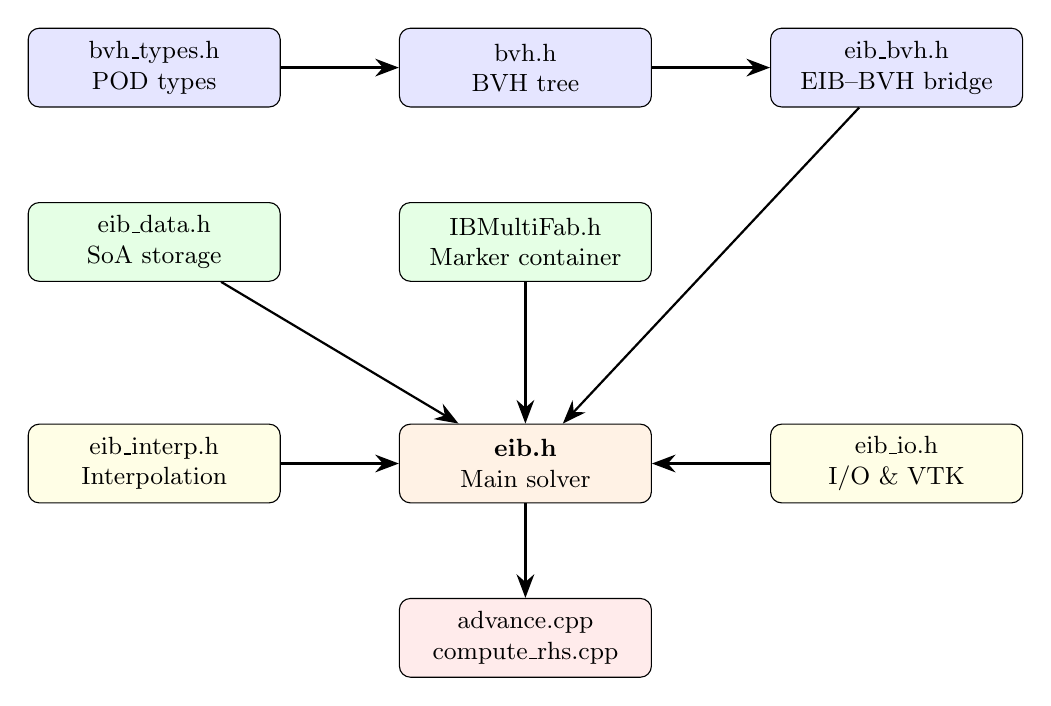
\begin{tikzpicture}[
    box/.style={draw, rounded corners, minimum height=1cm,
                minimum width=3.2cm, align=center, font=\small},
    arr/.style={-{Stealth[length=3mm]}, thick},
    node distance=1.2cm and 1.5cm
  ]
  % Top row: types
  \node[box, fill=blue!10] (types) {bvh\_types.h\\POD types};
  \node[box, fill=blue!10, right=of types] (bvh) {bvh.h\\BVH tree};
  \node[box, fill=blue!10, right=of bvh] (eib_bvh) {eib\_bvh.h\\EIB--BVH bridge};

  % Middle row: data + container
  \node[box, fill=green!10, below=of types] (data) {eib\_data.h\\SoA storage};
  \node[box, fill=green!10, right=of data] (ibmf) {IBMultiFab.h\\Marker container};

  % Bottom row: solver + helpers
  \node[box, fill=orange!10, below=1.8cm of ibmf] (eib) {\textbf{eib.h}\\Main solver};
  \node[box, fill=yellow!10, left=of eib] (interp) {eib\_interp.h\\Interpolation};
  \node[box, fill=yellow!10, right=of eib] (io) {eib\_io.h\\I/O \& VTK};

  % Caller
  \node[box, fill=red!8, below=of eib] (caller) {advance.cpp\\compute\_rhs.cpp};

  % Arrows
  \draw[arr] (types) -- (bvh);
  \draw[arr] (bvh) -- (eib_bvh);
  \draw[arr] (eib_bvh) -- (eib);
  \draw[arr] (data) -- (eib);
  \draw[arr] (ibmf) -- (eib);
  \draw[arr] (interp) -- (eib);
  \draw[arr] (io) -- (eib);
  \draw[arr] (eib) -- (caller);
\end{tikzpicture}
\end{center}

%==========================================================================
\section{New Files}
%==========================================================================

\begin{longtable}{p{3.5cm} p{1cm} p{9cm}}
\toprule
\textbf{File} & \textbf{Lines} & \textbf{Purpose} \\
\midrule
\texttt{bvh\_types.h} & 478
  & POD type definitions: \texttt{Point}, \texttt{Vec},
    \texttt{AABB}, \texttt{BVHNode}, \texttt{TriMesh} (3D),
    \texttt{Polygon2D} (2D), \texttt{SurfElem}, \texttt{LocalFrame},
    \texttt{ClosestPointResult}, \texttt{BoundedSide} enum.
    All types are GPU-annotated. \\

\texttt{bvh.h} & 524
  & BVH construction (Morton-code median split on CPU) and query
    (stack-based traversal on GPU).  Supports both \texttt{TriMesh}
    and \texttt{Polygon2D} geometries.  Core functions:
    \texttt{build()}, \texttt{closest\_point\_query()},
    \texttt{BVHQueryView} (POD capture for GPU lambdas). \\

\texttt{eib\_bvh.h} & 942
  & Bridge between EIB and BVH.  Key components:
    \begin{itemize}
      \item \texttt{InsideTester}/\texttt{InsideTesterView}: GPU inside/outside
            classification via 3-ray majority-vote (M\"oller--Trumbore).
      \item STL reader (ASCII + binary), OFF reader, 2D polygon reader.
      \item \texttt{build\_geometry\_cache()}: precompute \texttt{LocalFrame}
            and \texttt{SurfElem} arrays.
    \end{itemize} \\

\texttt{eib\_data.h} & 637
  & Compile-time constants (\texttt{MAX\_NGEOM}, interpolation thresholds,
    image-point scaling factors).
    SoA data structures:
    \texttt{gpData\_t} (ghost points),
    \texttt{surfImp\_t} (surface image points),
    \texttt{surfPhys\_t} (surface physical data),
    \texttt{FaceCSR} (compressed sparse row for per-FAB face iteration).
    SFINAE traits for wall-model dispatch. \\

\texttt{eib\_interp.h} & 519
  & Included inside \texttt{eib\_t} class body.  Functions:
    \texttt{valid\_mirror()},
    \texttt{search\_optimal\_image\_point()},
    \texttt{search\_image\_point()},
    \texttt{computeIPweights()} (bi-/tri-linear),
    \texttt{interpolateIMs()},
    \texttt{extrapolate()} (Lagrange, adaptive order),
    \texttt{global2local()}/\texttt{local2global()} frame transforms. \\

\texttt{eib\_io.h} & 544
  & Included inside \texttt{eib\_t} class body.  Functions:
    \texttt{read\_geom()} (master geometry loader),
    \texttt{plotSURF()} (VTK \texttt{.vtp} writer),
    \texttt{gatherSurfData()} (MPI gather to rank~0),
    \texttt{buildCSR()} (per-level face CSR). \\

\bottomrule
\end{longtable}

%==========================================================================
\section{Modified Files}
%==========================================================================

\subsection{\texttt{eib.h} --- Main Solver Class}

Reduced from $\sim$3800 to $\sim$1400 lines by extracting helpers into
the six new headers above.

Key new members and methods:

\begin{longtable}{p{5cm} p{9cm}}
\toprule
\textbf{Member / Method} & \textbf{Description} \\
\midrule
\texttt{gpstore\_a[level]}
  & Level-wide flattened ghost-point store (CSR-indexed by FAB).
    Contains \texttt{GPStoreView} (POD for GPU capture) and
    \texttt{GPStore} (owns \texttt{ManagedVector}). \\

\texttt{computeAllGPs()}
  & Single \texttt{ParallelFor} over all GPs on a level.  Uses
    \texttt{gpstore\_a} + device \texttt{Array4} pointers + FAB-offset
    mapping.  Replaces per-FAB \texttt{computeGPs()}. \\

\texttt{rebuildGeometryData()}
  & Recomputes BVH trees, inside/outside testers, bounding boxes,
    and surface-element caches after vertex positions change
    (moving geometry). \\

\texttt{geom\_a[ngeom]}
  & Explicit geometry storage (\texttt{TriMesh} or \texttt{Polygon2D}). \\

\texttt{bvh\_a[ngeom]}
  & BVH acceleration structures per geometry. \\

\texttt{inout\_fa[ngeom]}
  & \texttt{InsideTester} per geometry for inside/outside queries. \\

\texttt{faces\_per\_level}
  & CSR structure for efficient face iteration per level/FAB. \\
\bottomrule
\end{longtable}

\subsection{\texttt{IBMultiFab.h} --- Marker Container}

\begin{itemize}
  \item Explicit \texttt{delete} of copy constructors (prevent expensive
        deep-copies of \texttt{Gpu::ManagedVector}).
  \item Default move constructors enabled.
  \item \texttt{gpData} (ghost-point geometry) is NOT carried in alias
        constructors or FillBoundary --- it is local per-FAB data.
  \item Added \texttt{copytoRealMF()} for plotfile output.
\end{itemize}

\subsection{\texttt{ib\_walltypes.h} --- Wall Model Parameters}

\begin{itemize}
  \item Added \texttt{interior\_is\_solid} flag to \texttt{ibmparm\_t}.
  \item Extended \texttt{compute\_surfIB} to 7-argument signature
        matching the new \texttt{eib.h} surface computation interface.
  \item Added \texttt{const int\&} helper overload for SFINAE trait
        detection without call-site ambiguity.
\end{itemize}

\subsection{\texttt{eib\_cgal.h} --- CGAL Wrappers}

\begin{itemize}
  \item New BVH-based inside/outside testing functions alongside existing
        CGAL paths.
  \item Closest-point queries extended for the BVH code path.
  \item Retained CGAL as optional high-accuracy fallback.
\end{itemize}

%==========================================================================
\section{GPStore Architecture}
%==========================================================================

\subsection{Data Layout}

Ghost points are stored in a flat CSR (Compressed Sparse Row) structure
per AMR level:

\begin{lstlisting}[caption={GPStore CSR layout}]
struct GPStoreView {   // POD, GPU-capturable
    int*  gp_fab;        // gp_fab[ii] = local FAB index for GP ii
    int*  fab_offsets;   // fab_offsets[f] = start index of FAB f
    // ... per-GP fields (xyz, ijk, normals, weights, etc.)
};

struct GPStore {        // owns Gpu::ManagedVector storage
    Gpu::ManagedVector<int> gp_fab_v;
    Gpu::ManagedVector<int> fab_offsets_v;
    // ...
    void allocate();    // resize after gp_counts known
    GPStoreView view(); // return POD for GPU capture
};
\end{lstlisting}

\subsection{Three-Phase Workflow}

The GPStore enables a three-phase workflow that replaces the old per-FAB
\texttt{computeGPs()}:

\begin{enumerate}
  \item \textbf{Phase 1 --- cons2prims:}
    Fill a level-wide \texttt{prims\_mf} MultiFab from the conservative
    state (one \texttt{MFIter} loop).

  \item \textbf{Phase 2 --- computeAllGPs:}
    Single \texttt{ParallelFor} over all GPs on the level.  Each GP
    reads from the correct FAB via \texttt{gp\_fab[ii]} mapping and
    \texttt{fab\_offsets} offset.

  \item \textbf{Phase 3 --- prims2cons:}
    Convert primitives back to conservatives at GP cells only (one
    \texttt{MFIter} loop, only cells with \texttt{ibMarkers(i,j,k,1)}).
\end{enumerate}

This pattern is used in both \texttt{advance.cpp} (post-Runge--Kutta
correction) and \texttt{compute\_rhs.cpp} (pre-flux computation).

%==========================================================================
\section{Moving Geometry Support}
%==========================================================================

For moving immersed boundaries, the following sequence is executed at the
start of each time step in \texttt{advance.cpp}:

\begin{lstlisting}[caption={Moving geometry update sequence}]
#ifdef AMREX_USE_GPIBM
if (CNS::ib_move) {
    // 1. User callback updates vertex positions
    PROB::update_geometry(time + dt, IBM::ib.geom_a, IBM::ib.ngeom);
    // 2. Rebuild BVH, inside/outside testers, surface cache
    IBM::ib.rebuildGeometryData();
    // 3. Recompute markers and GP data on all levels
    rebuildIBM();
}
#endif
\end{lstlisting}

\texttt{rebuildGeometryData()} performs:
\begin{enumerate}
  \item Rebuild BVH trees from updated vertex positions.
  \item Reconstruct \texttt{InsideTester} for each geometry.
  \item Recompute bounding boxes.
  \item Rebuild \texttt{LocalFrame} and \texttt{SurfElem} caches.
\end{enumerate}

%==========================================================================
\section{Integration with \texttt{compute\_rhs.cpp}}
%==========================================================================

The main changes in \texttt{compute\_rhs.cpp} for the IBM refactor:

\begin{longtable}{p{4.5cm} p{9cm}}
\toprule
\textbf{Change} & \textbf{Detail} \\
\midrule
Compile guard
  & \texttt{\#error} if both \texttt{AMREX\_USE\_GPIBM} and
    \texttt{CNS\_USE\_EB} are defined. \\

GPStore pre-loop
  & Level-wide \texttt{cons2prims()} + \texttt{computeAllGPs()} before
    the MFIter loop. \\

Prims aliasing
  & Inside the loop, \texttt{prims} aliases \texttt{prims\_mf.array(mfi)}
    (no per-FAB allocation when IBM is active). \\

geoMarkers alias
  & Direct \texttt{Array4} alias to \texttt{IBMultiFab} markers;
    eliminates the old auxiliary \texttt{BaseFab<uint8\_t>} +
    \texttt{ParallelFor} copy. \\

Solid RHS zeroing
  & Uses explicit \texttt{if (geoMarkers != 0)} branch instead of
    \texttt{state *= (1 - int(marker))} multiplication. \\
\bottomrule
\end{longtable}

%==========================================================================
\section{Known TODOs}
%==========================================================================

\begin{itemize}
  \item \texttt{computeSURFs} in \texttt{postCoarseTimeStep} is commented
        out --- needs re-enabling with GPStore.
  \item \texttt{rz\_geometric\_source\_ibm} is not implemented
        (RZ + IBM combination).
  \item ``Pure virtual method called'' crash at program exit (pre-existing,
        likely destruction-order issue with AMReX/IBM singletons).
\end{itemize}

\end{document}
